\section{Problem 3}
\textit{Explain the connection – if possible- between table 2.6 and figure 2.58 in Mobile Antenna System Handbook on page 103-4 – the experimental results}\\

\begin{center}
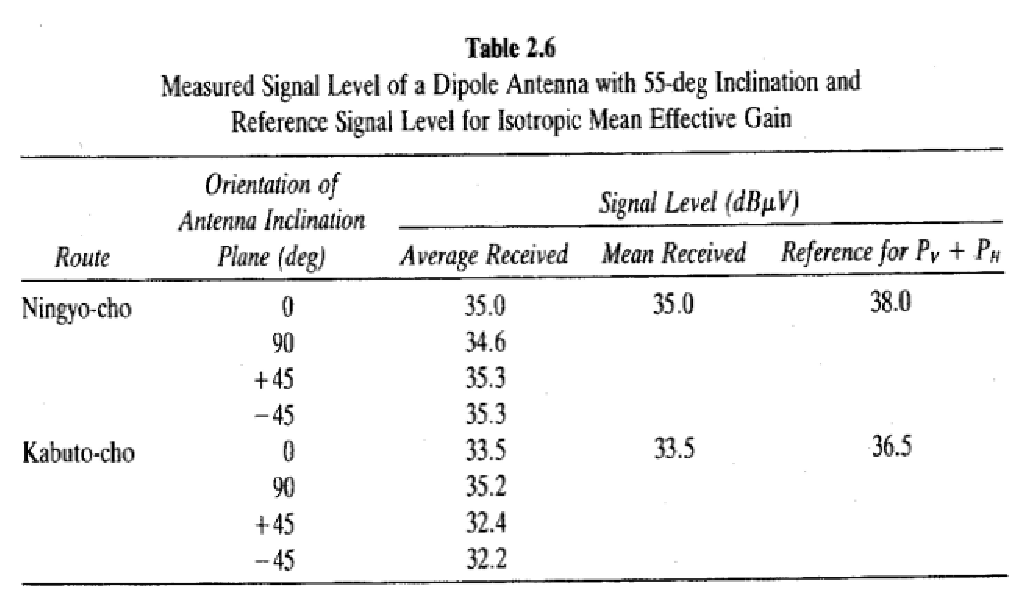
\includegraphics[scale=0.6]{figures/Tabel_2_6.eps}\\
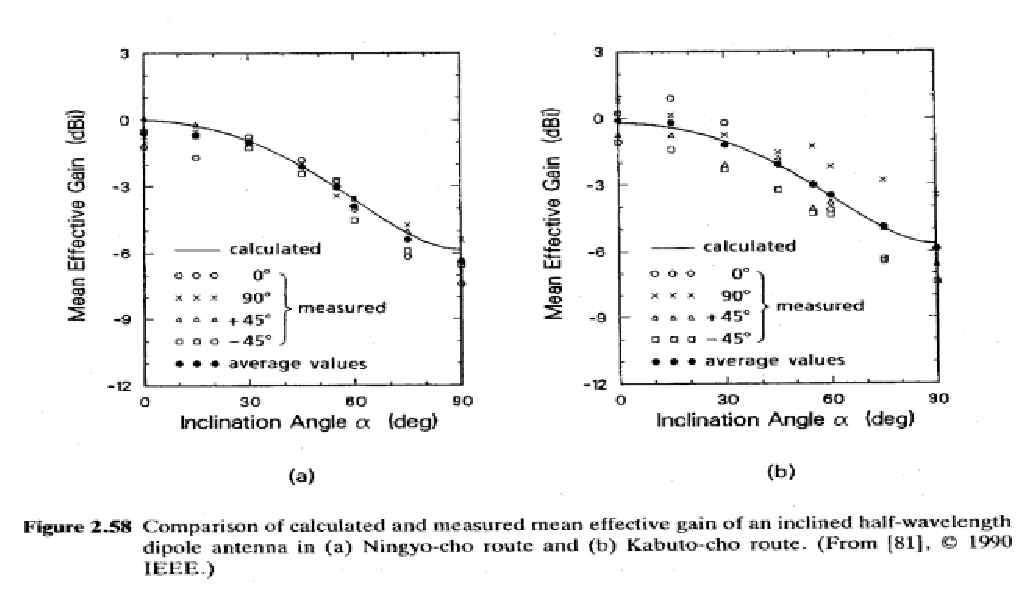
\includegraphics[scale=0.85]{figures/Figure_2_58.eps}
\end{center}

% I THINK IS BETTER NOT TO INCLUDE THE TABLE AND THE FIGURE AS LOCAL FIGURES SO IS EASIER FOR REFERRING AND MORE CLEAR TO UNDERSTAND

%Table 2.6 from the book is shown in \figref{fig:Tabel_2_6}:
%\fig[keepaspectratio=true,width=14cm]{Tabel_2_6.eps}{Table 2.6 from Mobile Antenna Systems Handbook }{fig:Tabel_2_6}
%Figure 2.58 from the book is shown in \figref{fig:Figure_2_58}:
%\fig[keepaspectratio=true,width=16cm]{Figure_2_58.eps}{Table 2.6 from Mobile Antenna Systems Handbook}{fig:Figure_2_58}
Table 2.6 shows the numeric results of the received signal level of a dipole antenna in the same locations with fixed inclination of 55° and different orientation. The result is given for the two routes - Ningyo-cho and Kabuto-cho. The average received signal level is given for the four different orientations (0 90 +45 -45) and the mean of these. Also given is the reference $P_V + P_H$, and the Mean Effective Gain (MEG) can be calculated by equation \ref{eq1:mm3_pb3} and with the results given in dB $G_{e}dB = P_{rec}dB - (P_{V}dB + P_{H}dB)$. 
\begin{flalign}\label{eq1:mm3_pb3}
&& G_e &= \frac{P_{rec}}{P_V + P_H} &
\end{flalign}
In figure 2.58 the MEG are shown for different inclination and different orientation. In 2.58a the result for the Ningyo-cho route and 2.58b for the Kabuto-cho route. From the figure it can be seen that the Kabuto-cho route have a higher deviation in comparison to the Ningyo-cho route. 


% 
% shows the results of the  of an antenna in two different cities as a function of the inclination of the antenna dipole, and the orientation of the respective inclination plane (0,+45,-45,90).
%  
% 
%  
% 
% The inclination of the antenna was fixed to  in order to get the reference for the $P_V + P_H$ (With this inclination the $P_{rec}$ is half of that independently from the XPR). Then it is measured the received signal while rotating the orientation of the antenna inclination plane. As the MEG is defined as:



% Thus, it can be easily obtained the MEG for each orientation values by just subtracting the reference $P_V + P_H$ to each received power. Those MEG values correspond to the points showed in the figure 2.58 for $\alpha$=55.
